\documentclass{beamer}
 
\usepackage[utf8]{inputenc}
\usepackage[brazil]{babel} % pacote portugues brasileiro
\usepackage{textpos}
\usepackage{hyperref}
\definecolor{blue(pigment)}{rgb}{0.2, 0.2, 0.6}
\hypersetup{
    colorlinks=true,
    linkcolor=blue(pigment),
    filecolor=magenta,      
    urlcolor=cyan,
}

\usepackage{verbatim}
%\usetheme{Boadilla}
\usetheme{Montpellier}
\usecolortheme{rose}
% \graphicspath{fig/aula1}
% Layout da pagina
\hypersetup{pdfpagelayout=SinglePage}
 
%Information to be included in the title page:
\title[Apresentação da Disciplina]{Introdução a páginas WEB}
 \subtitle{Disciplina: Desenvolvimento de Sistemas com PHP}
\author{Juliana C. Silva}
\institute{Universidade Positivo}
%\date{10 de março de 2021}
\definecolor{UniGray}{RGB}{192,192,192}
\definecolor{nGray}{RGB}{220,220,220}

\setbeamercolor{block title}{use=structure,bg=UniGray}
\setbeamercolor{block body}{use=structure,bg=nGray}
\setbeamersize{text margin left=25pt,text margin right=25pt}
\setbeamertemplate{navigation symbols}{}%remove navigation symbols
 
% Configurando layout para mostrar codigos C++
\usepackage{listings}
\lstset{
  language=HTML,
  basicstyle=\ttfamily\small, 
  keywordstyle=\color{blue}, 
  stringstyle=\color{red}, 
  commentstyle=\color{red}, 
  extendedchars=true, 
  showspaces=false, 
  showstringspaces=false, 
  numbers=left,
  numberstyle=\tiny,
  breaklines=true, 
  backgroundcolor=\color{green!10},
  breakautoindent=true, 
  captionpos=b,
  xleftmargin=0pt,
}

\begin{document}
%------------------------------------------------------------------------------------------
\frame{\titlepage}
 
\addtobeamertemplate{frametitle}{}{%
\begin{textblock*}{100mm}(.8\textwidth,-1.45cm)
\end{textblock*}
}

%-----------------------------------------------------------------------------------------
\section{A disciplina}
\begin{frame}{Começando...}
  \begin{itemize}
   \item Prof. Juliana Costa Silva
    \item E-mail: juliana.silva@up.edu.br
    \item Quem é a professora?
    \pause \item \textcolor{red}{Como a professora trabalha??}
  \end{itemize}
\end{frame}
%--------------------------------------------------------------------------------------
\begin{frame}{Começando [2]}
  \begin{itemize}
   \item Plano de aulas (Disponível para leitura);
    \item Trabalhos ;
    \item Avaliação: datas no plano de aulas (disponível no Blackcboard);
  \end{itemize}
\end{frame}
%--------------------------------------------------------------------------------------
\begin{frame}{O que veremos?}
  \begin{itemize}
   \item HTML + CSS (básico);
        \begin{itemize}
            \item estrutura de páginas WEB;
            \item Tags básicas HTML + Formulários;
            \item Cores, formatação e posicionamento de elementos;
        \end{itemize}
    \item PHP: 
        \begin{itemize}
            \item Variáveis;
            \item Estruturas de decisão;
            \item Estruturas de repetição;
            \item Funções;
            \item GET, POST;
            \item Formulários WEB;
            \item Processando informações com PHP;
            \ietm Conexão com banco de dados;
        \end{itemize}
  \end{itemize}
\end{frame}

%------------------------------------------------------------------------------------------
\begin{frame}
\frametitle{Roteiro} % Table of contents slide, comment this block out to remove it
\tableofcontents % Throughout your presentation, if you choose to use \section{} and \subsection{} commands, 
%these will automatically be printed on this slide as an overview of your presentation
\end{frame}
%---------------------------------------------------------------------------------
\section{Introdução}
\begin{frame}{Sobre a WEB}
  \begin{enumerate}
    \item Como tantas informações ficam disponíveis na internet?
    \item Descreva em \textbf{3 palavras} o funcionamento de uma página WEB.
  \end{enumerate}
  \begin{center}

\includegraphics[height=0.5\paperheight]{fig/aula1/mentimeter_profcostasilvati_qr_code.png} \\
    		Acesse o questionário online ou o link ( \href{https://www.menti.com/47mtir9zhw}{https://www.menti.com/47mtir9zhw}).
		\end{center}
\end{frame}
%---------------------------------------------------------------------------------------
\begin{frame}{Exibindo páginas WEB}
		\begin{center}
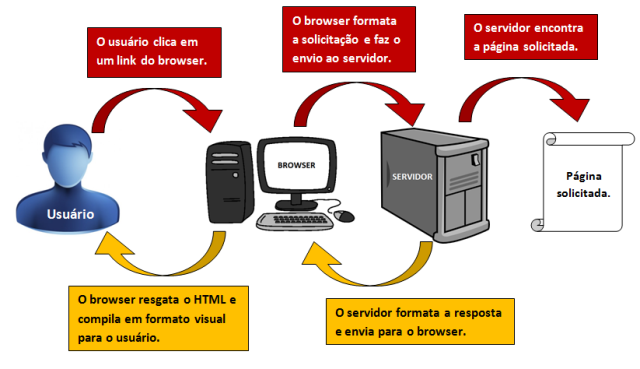
\includegraphics[height=0.65\paperheight]{fig/aula1/funcionamentoweb.jpg} \\
    		\tiny \textbf{Fonte:} \cite{freeman2008use}.
		\end{center}
\end{frame}
%---------------------------------------------------------------------------------
\begin{frame}{Exibindo páginas WEB}
  Como o navegador sabe o que exibir?
  \begin{block}{HTML}
    \begin{itemize}
      \item HTML - Hipertext Markup Language (Linguagem de Marcação de 
Hipertexto);
       \item Isto significa que é um código utilizado para descrever a 
estrutura de um documento, mas não é a verdadeira apresentação dele.
       \item O HTML diz ao navegador, tudo sobre o conteúdo recebido, e 
a estrutura da página;
       \item O HTML define cabeçalhos, parágrafos, listas, tabelas entre 
muitos outros elementos, por meio de marcas (\textit{tags}).
    \end{itemize}
    \tiny{Fonte: \cite{marinho2016}}
  \end{block}
\end{frame}
%---------------------------------------------------------------------------------
\section{HTML}
\begin{frame}{Tags HTML}
  \begin{center}
    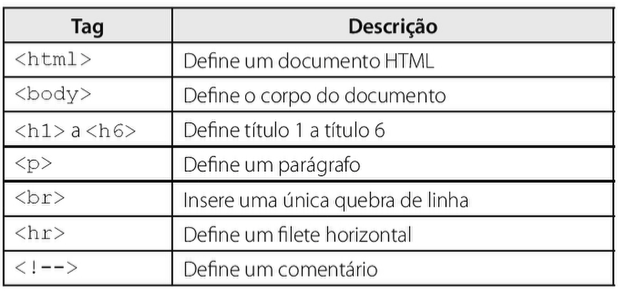
\includegraphics[height=0.5\paperheight]{fig/aula1/tagBasica.png}\\
    \tiny{Fonte: \cite{marinho2016}.}
   \end{center}
\end{frame}
%---------------------------------------------------------------------------------
\begin{frame}{HTML}
  O navegador lê o código HTML e, interpreta todas as \textit{tags}. \\
   \textbf{tags:} Palavras entre os sinais de maior e menor, como: 
$<head>$ ou $<p>$.
\end{frame}
%----------------------------------------------------------------
\begin{frame}{Estrutura}
  \begin{block}{Estrutura de uma página HTML}
    Toda página html, por mais simples que seja, deve conter as seguintes tags 
elementares:
    \begin{itemize}
     \item $<html>$: é a tag que identifica o documento como um hipertexto html;
     \item $<head>$: é a tag que apresenta informações gerais sobre a 
página e de configuração;
     \item $<title>$: é a tag que informa o título de uma página na barra 
do navegador;
     \item $<body>$: é a tag que delimita o conteúdo da página;
  \end{itemize}
  \end{block}
\end{frame}
%----------------------------------------------------------------
\begin{frame}{Estrutura II}
  \begin{block}{Estrutura de uma página HTML}
   \begin{itemize}
    \item Além disso, a tag a seguir define a codificação de caracteres 
para o padrão UTF-8: $<$meta charset = “UTF-8” $/>$ \\
   \item A instrução a seguir indica para o navegador utilizar a versão 
mais recente do HTML (HTML5):
  \item $<$!DOCTYPE html$>$
  \end{itemize}
  \end{block}
\end{frame}
%---------------------------------------------------------------------------------
\begin{frame}{HTML}
  Crie sua primeira página HTML. Abra o bloco de notas e salve um arquivo em 
branco com o nome exercicio1.html

  \begin{center}
    \lstinputlisting{fig/aula1/exercicio1.html}
  \end{center}
\end{frame}
%---------------------------------------------------------------------------------
\begin{frame}{Tag: Títulos}
  \begin{columns}
    \begin{column}{0.5\textwidth}
      Para indicar que um texto é um título em nossa página,
utilizamos a tag de heading;\\

      São tags de conteúdo e vão de $<$h1$>$ até $<$h6$>$;\\
 
    A variação entre as tags de heading definem o grau de destaque do texto;
   \end{column}
   \begin{column}{0.4\textwidth}
    \begin{center}
      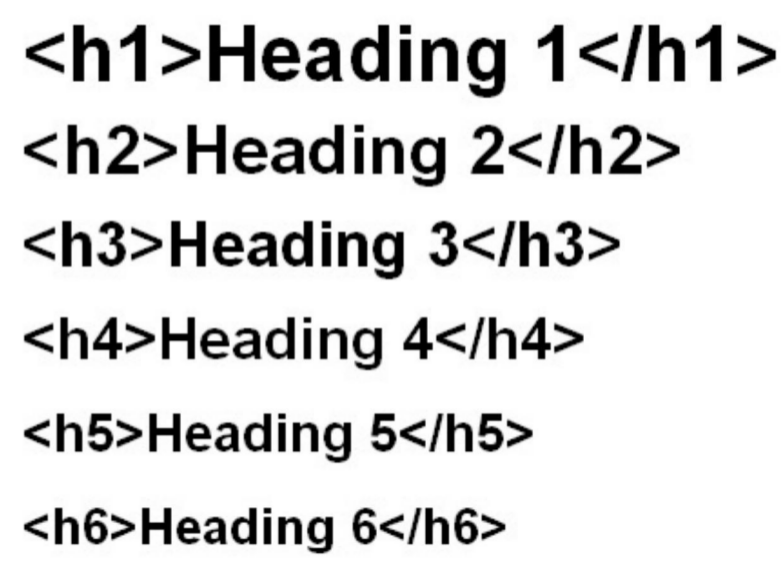
\includegraphics[height=0.4\paperheight]{fig/aula1/heading.png} \\
    \end{center}
   \end{column}
  \end{columns}
  
  Acrescente Três títulos a sua página!
\end{frame}
%-------------------------------------------------------------------------
\begin{frame}{Resultado}
  \begin{center}
    \lstinputlisting{fig/aula1/exercicio2.html}
  \end{center}
\end{frame}
%-------------------------------------------------------------------------
\begin{frame}{Tags de formatação}
 As seguintes tags são utilizadas para a apresentação de conteúdo textual em 
uma 
página:
\begin{itemize}
 \item $<$p$>$: tag para a representação de um parágrafo;
  \item $<$span$>$: tag para representar um texto sem significado (deve 
ser usado quando nenhum outro elemento de texto semântico representar um 
significado adequado);
   \item Outros;
\end{itemize}
\end{frame}
%-------------------------------------------------------------------------
\begin{frame}{Tags de texto}
 Teste as Tags abaixo no seu arquivo html e descreva o que cada uma faz
\begin{itemize}
 \item $<$strike$>$
  \item $<$sub$>$
  \item $<$sup$>$
  \item $<$big$>$
  \item $<$small$>$
  \item $<$tt$>$
  \item $<$pre$>$
  \item $<$cite$>$
  \item $<$strong$>$
  \item $<$em$>$
  \item $<$blockquote$>$
  \item $<$q$>$
\end{itemize}
\end{frame}
%-----------------------------------------------------------
\begin{frame}{Detalhando...}
 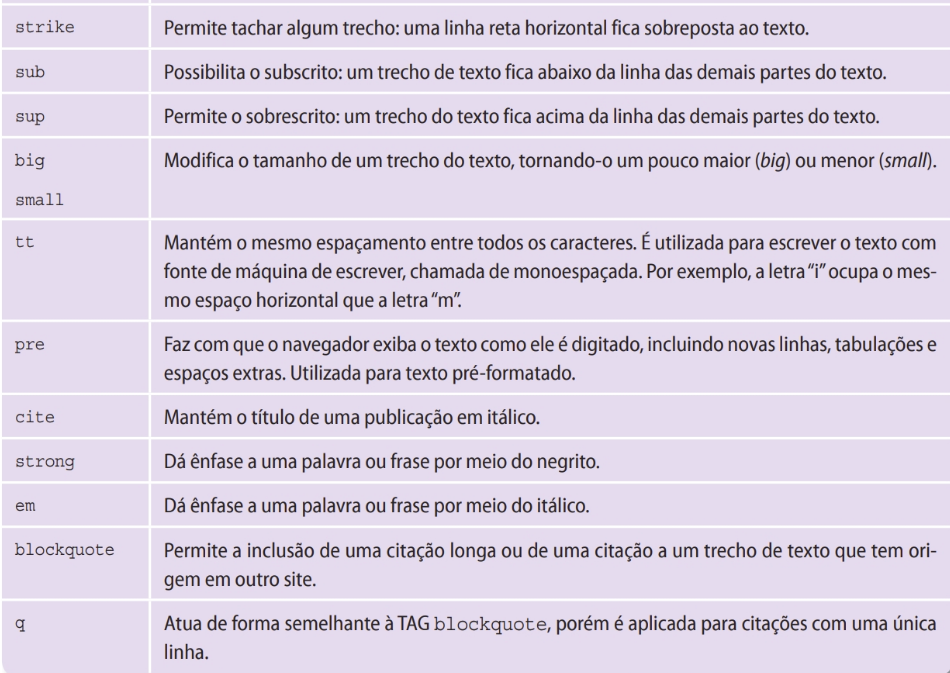
\includegraphics[height=0.7\paperheight]{fig/aula1/tagFormata.png} \\
\end{frame}
%----------------------------------------
\begin{frame}{Livros da disciplina}
Disponíveis em Aluno Online $>$ Biblioteca $>$ \textcolor{red}{E-books - Minha Biblioteca} 
\begin{columns}
    \begin{column}{0.4\textwidth}
    \center
    PHP na Prática\\
     
\includegraphics[height=0.5\paperheight]{fig/aula1/silva2016php.png} \\
     \cite{silva2016php}
    \end{column}
    \begin{column}{0.4\textwidth}
    \center
    Desenvolvimento de Sistemas com PHP\\
     
\includegraphics[height=0.4\paperheight]{fig/aula1/saraiva2018php.png} \\
     \cite{saraiva2018php}
    \end{column}
\end{columns}
\end{frame}
%---------------------------------------------------------------------------

\section{Referências}
\begin{frame}{Referências}%[allowframebreaks]
\frametitle{Referências}
\small
\begin{center}
\tiny
\bibliographystyle{apalike}
\bibliography{ref_aula}
\end{center}
\end{frame}
 
\end{document}
